\documentclass{beamer}

\usepackage[english]{babel}
\usepackage{url}
\usepackage{amsmath}

\usepackage[utf8]{inputenc}

\definecolor{gris}{rgb}{0.92,0.92,0.92}
\definecolor{blau-upc}{rgb}{.192,.365,.506}

\setbeamercolor{titlelike}{fg=blau-upc}
% \setbeamercolor{barra}{bg=white,fg=white}
\setbeamercolor{capcalera}{bg=blau-upc,fg=white}
\setbeamercolor{section in toc}{fg=blau-upc}
\setbeamertemplate{sections/subsections in toc}[circle]
\setbeamertemplate{itemize items}[circle]
\setbeamercolor{item}{fg=blau-upc}
\setbeamertemplate{blocks}[rounded][shadow=true]
\setbeamercolor*{block body}{bg=gris}
\setbeamerfont{block body}{size=\footnotesize}
\setbeamercolor*{block title}{parent=structure,bg=blau-upc,fg=white}

\setbeamersize{text margin left=12mm,text margin right=12mm}
\setbeamertemplate{navigation symbols}{}

\defbeamertemplate*{headline}{infolines theme}
{
	\begin{beamercolorbox}[wd=\paperwidth,ht=9.5mm,right]{white}%
		
\includegraphics[height=8mm]{./logotips/imperiallogo.pdf}\hspace*{1mm}\vskip0.2ex
	\end{beamercolorbox}
% 	\begin{beamercolorbox}[wd=\paperwidth,ht=0.5mm,left]{barra}%
% 		\hspace*{1mm}
% 	\end{beamercolorbox}
}

\setbeamertemplate{footline}
{
	\hbox{
	\begin{beamercolorbox}[wd=0.1\paperwidth,ht=10mm,left]{}
% 		\hspace*{1ex}
\includegraphics[height=8mm]{./logotips/imperiallogo.pdf}\vskip 2ex
	\end{beamercolorbox}
	\begin{beamercolorbox}[wd=0.8\paperwidth,ht=3ex,center]{}
		\hspace*{4ex}\insertsection\vskip 4ex
	\end{beamercolorbox}
	\begin{beamercolorbox}[wd=0.1\paperwidth,ht=3ex,right]{}
		\insertpagenumber\hspace*{6ex}\vskip 4ex
	\end{beamercolorbox}
	}
}

\setbeamertemplate{title page}
{
	\vbox{}
	\vfill
	\begin{centering}
		{\usebeamerfont{title}\usebeamercolor[fg]{title}\inserttitle}
		\vskip0.2em
		{\usebeamerfont{subtitle}\usebeamercolor[fg]{subtitle}\insertsubtitle}
		\vskip2em\par
		\small\insertauthor\par
		\vskip0.7em\par
		\tiny\insertdate\vskip1em\par
	\end{centering}
% 	\vfill
}

\usebackgroundtemplate{\put(-50,-340){
\includegraphics[width=10cm]{./logotips/imperialback.png}}} 

\title{NGS data: Beauty and the Beast}
\subtitle{{\it How to infer population genetics parameters from messy sequencing data}}
\author{Matteo Fumagalli}
\date{$12^{th}$ September 2017}

\begin{document}

\frame{\titlepage} 

%%%%%%%%%%%%%%%%%%%%%%%%%%%%%%%%%%%%%%%%%%%%%%%%%%%%%%

\frame{
\frametitle{Goal of the day}

	\begin{figure}
		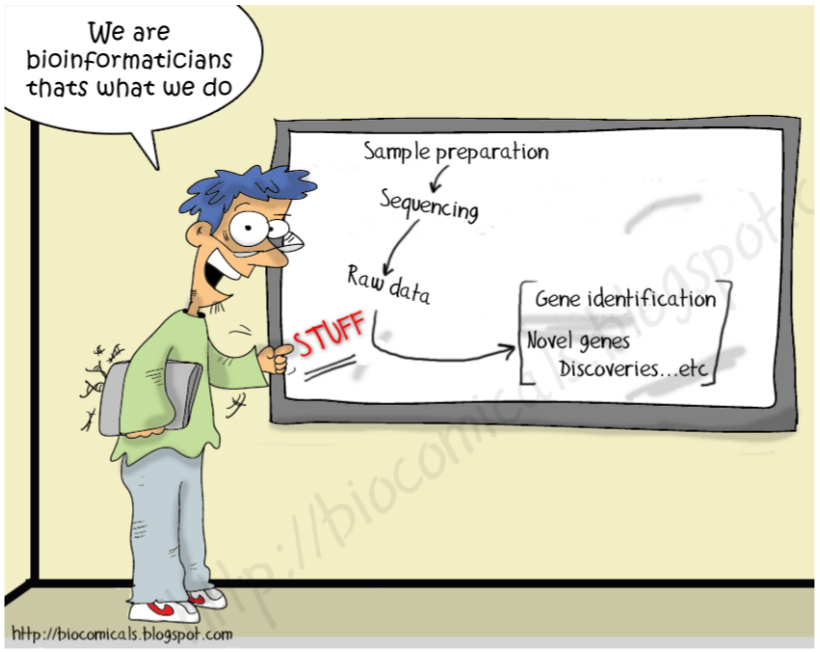
\includegraphics[scale=0.3]{Pics/bioinfo}
	\end{figure}

}

%%%%%%%%%%%%%%%%%%%%%%%%%%%%%%%%%%%%%%%%%%%%%%%%%%%%%%

\frame{\frametitle{Presentation outline}\tableofcontents}

%%%%%%%%%%%%%%%%%%%%%%%%%%%%%%%%%%%%%%%%%%%%%%%%%%%%%%

% data and issues
\section{Introduction}

%%%%%%%%%%%%%%%%%%%%%%%%%%%%%%%%%%%%%%%%%%%%%%%%%%%%%%

\frame{\frametitle{Sanger sequencing}

aka first/former generation sequencing

\begin{columns}

	\column{0.3\textwidth}

		\begin{figure}
			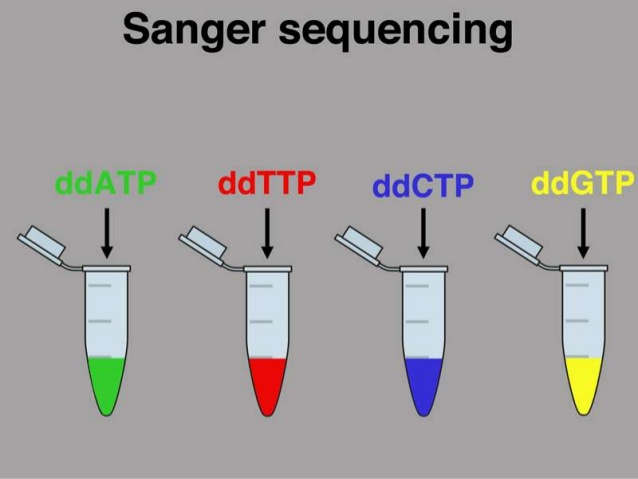
\includegraphics[scale=0.15]{Pics/sanger}
		\end{figure}

	\column{0.7\textwidth}

		\begin{figure}
			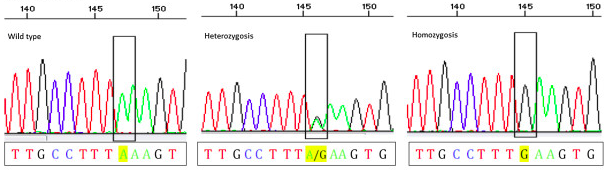
\includegraphics[scale=0.35]{Pics/sangerElectro}
		\end{figure}

\end{columns}

}

%%%%%%%%%%%%%%%%%%%%%%%%%%%%%%%%%%%%%%%%%%%%%%%%%%%%%%

\frame{\frametitle{Next Generation Sequencing}

	\begin{figure}
		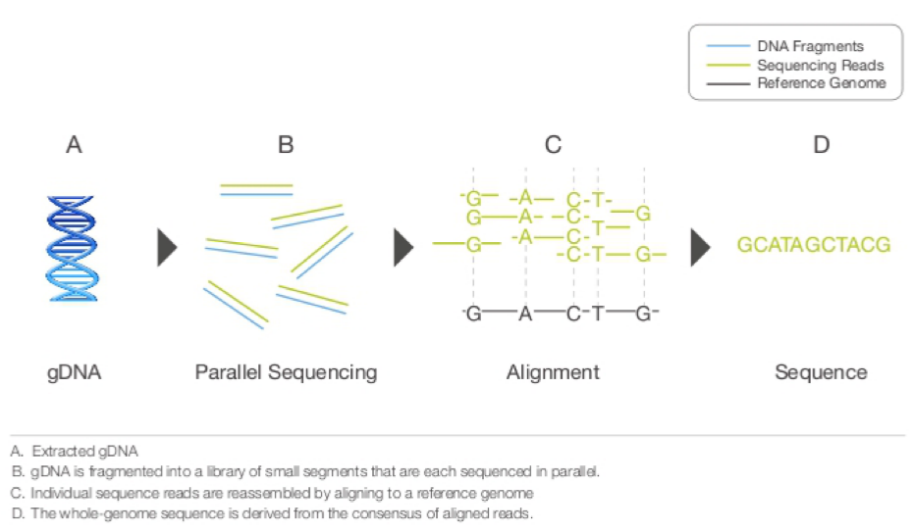
\includegraphics[scale=0.3]{Pics/illumina}
	\end{figure}

}


%%%%%%%%%%%%%%%%%%%%%%%%%%%%%%%%%%%%%%%%%%%%%%%%%%%%

\begin{frame}
\frametitle{Low-level data}

	\begin{figure}
                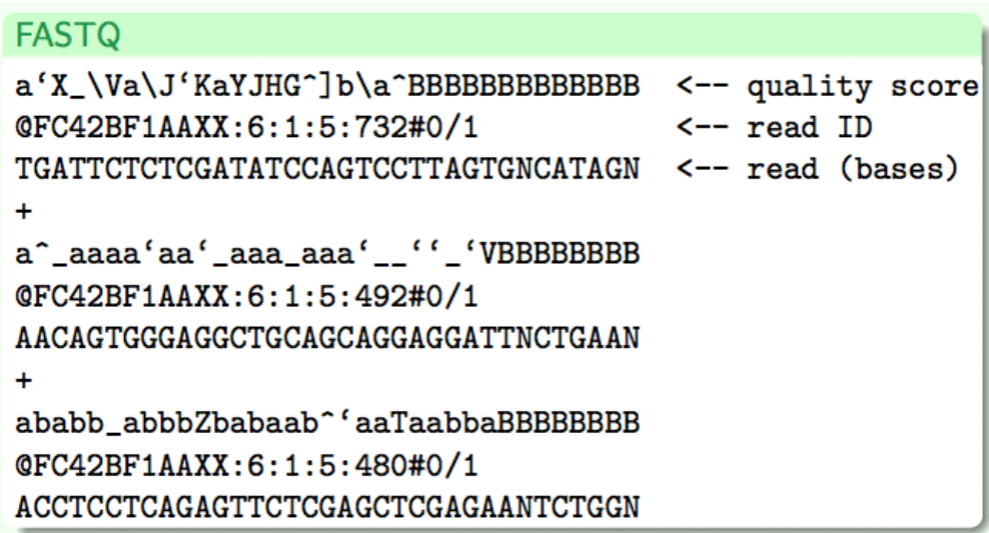
\includegraphics[width=\textwidth]{Pics/fastq.png}
        \end{figure}

\end{frame}



%%%%%%%%%%%%%%%%%%%%%%%%%%%%%%%%%%%%%%%%%%%%%%%%%%%%

\begin{frame}
\frametitle{Quality scores}

        \begin{figure}
                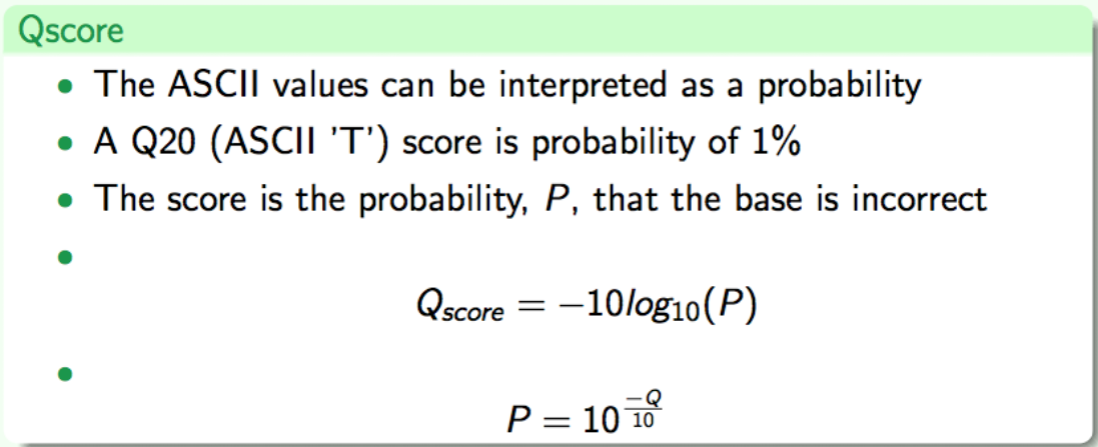
\includegraphics[width=\textwidth]{Pics/qscores.png}
        \end{figure}

\end{frame}

%%%%%%%%%%%%%%%%%%%%%%%%%%%%%%%%%%%%%%%%%%%%%%%%%%%%

\begin{frame}
\frametitle{Quality scores}

	The qscores are encoded as ASCII characters, and are shifted by +33 (now the standard) or +64.

        \begin{figure}
                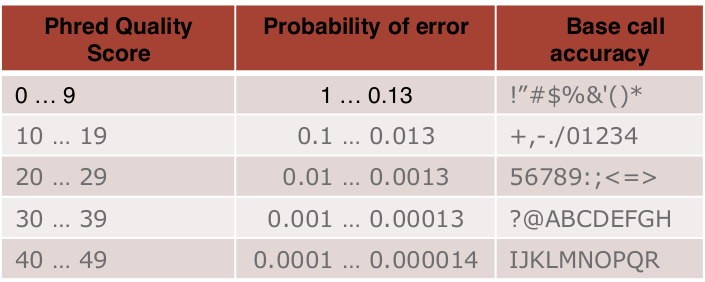
\includegraphics[width=\textwidth]{Pics/qscores_table.png}
        \end{figure}

\end{frame}

%%%%%%%%%%%%%%%%%%%%%%%%%%%%%%%%%%%%%%%%%%%%%%%%%%%%%

\begin{frame}
\frametitle{Quality scores}

	\begin{block}{Example}
		From a fastq file we observe an `A` with a qscore encoded as `7`.
		What is the probability of being `A`? What is the probability of geing `G`? 
	\end{block}

	\begin{enumerate}
		\item We find that the corresponding ASCII value of `7` is ? (hint: \url{http://www.asciitable.com})
		\pause
		\item We substract 33 to get a value of ?. This is our qscore.
		\item The probability of `A` being incorrect is ? (hint: $p=10^\frac{-Q}{10}$)
		\item The probability of `A` being correct is ?
		\item The probability of being `G` (or `C` or `T`) is ?
	\end{enumerate}

\end{frame}

%%%%%%%%%%%%%%%%%%%%%%%%%%%%%%%%%%%%%%%%%%%%%%%%%%%%%

\begin{frame}
\frametitle{FastQ files}

        \begin{figure}
                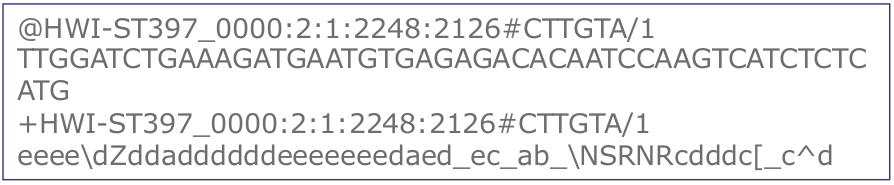
\includegraphics[width=\textwidth]{Pics/fastq_more.png}
        \end{figure}

	\begin{itemize}
		\item sequencer
		\item flowcell
		\item lane/cell/tile
		\item position within the tile
		\item barcode id for pooling/multiplexing
		\item pair
		\item ...
	\end{itemize}

\end{frame}

%%%%%%%%%%%%%%%%%%%%%%%%%%%%%%%%%%%%%%%%%%%%%%%%%%%%%

\begin{frame}
\frametitle{Quality check of fastq files: fastQC}

        \begin{figure}
                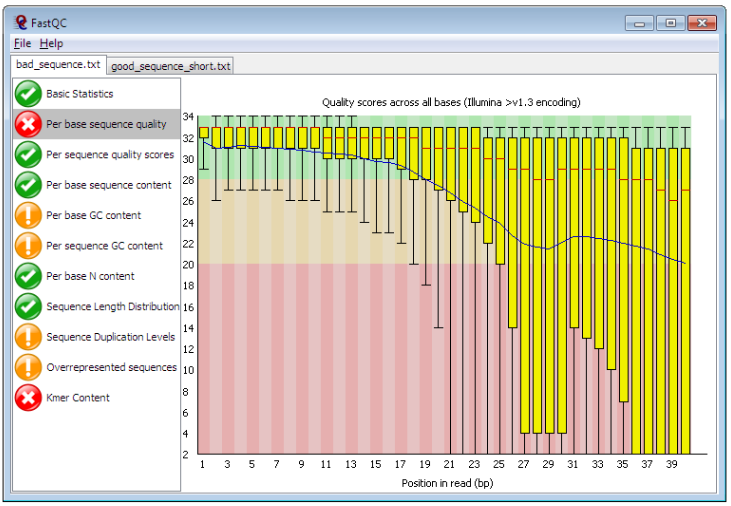
\includegraphics[width=0.7\textwidth]{Pics/fastqc.png}
        \end{figure}

	\tiny{
	\begin{itemize}
		\item distribution of qscores over read
		\item overrepresented kmers
		\item ...
	\end{itemize}
	}

	\begin{center}
		\footnotesize{\url{http://www.bioinformatics.babraham.ac.uk/projects/fastqc/}}
	\end{center}

\end{frame}

%%%%%%%%%%%%%%%%%%%%%%%%%%%%%%%%%%%%%%%%%%%%%%%%%%%%%%

\begin{frame}
\frametitle{Alignment of reads}

        \begin{figure}
                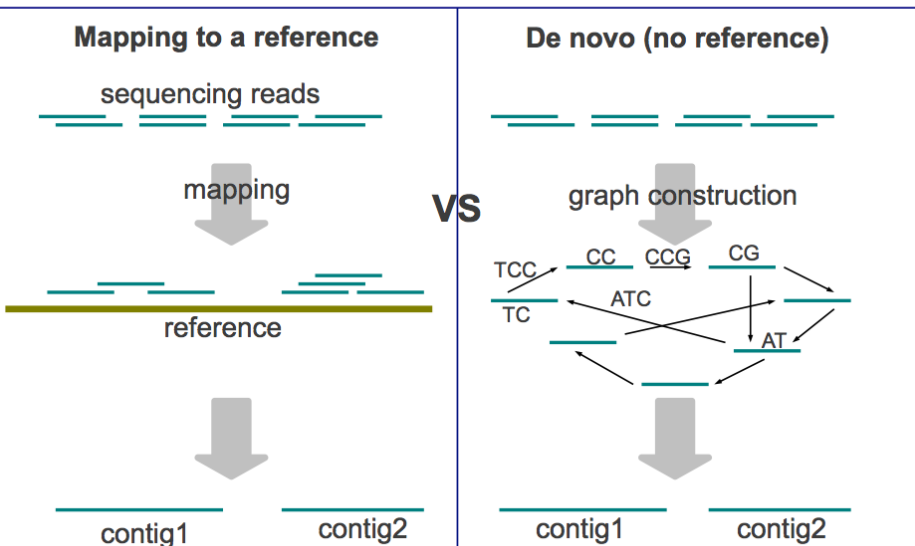
\includegraphics[width=\textwidth]{Pics/mapping.png}
        \end{figure}

\end{frame}

%%%%%%%%%%%%%%%%%%%%%%%%%%%%%%%%%%%%%%%%%%%%%%%%%%%%%

\begin{frame}
\frametitle{Mapping to a reference}

	Issues:\\
	(i) Millions of short reads.\\
	(ii) Blat/blast is too slow.\\
	But:\\
	Mate-pair gives additional information.\\

	Many aligners exists:
	\begin{itemize}
		\item Soap/soap2 (BGI)
		\item Maq/bwa (Heng Li)
		\item Bowtie/bowtie2 (Langmead B)
		\item Eland, SSAHA2,RMAP,shrimp,zoom,GEM, snap, novoAlign.
	\end{itemize}
	Most are based on burrows wheeler transform BTW (BWA,Bowtie,Soap2,...)

\end{frame}

%%%%%%%%%%%%%%%%%%%%%%%%%%%%%%%%%%%%%%%%%%%%%%%%%%%%%

\begin{frame}
\frametitle{Mapping to a reference}

	Many different aligners, what's the difference?

	\begin{itemize}
		\item Memory usage
		\item Speed
		\item Gapped (indels)
		\item Using qscores (bwa pssm)
		\item Estimating a \textbf{mappability score}
		\item Multiple best hits
		\item Paired end data
		\item Output \textbf{formats} (SAM,...)
	\end{itemize}

\end{frame}

%%%%%%%%%%%%%%%%%%%%%%%%%%%%%%%%%%%%%%%%%%%%%%%%%%%%%%

\begin{frame}
\frametitle{Alignment file}

        \begin{figure}
                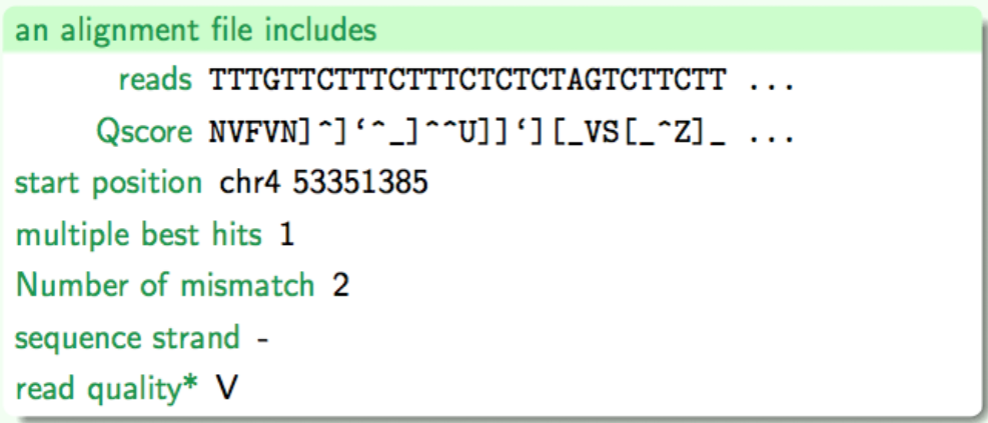
\includegraphics[width=\textwidth]{Pics/mapping_file.png}
        \end{figure}

\end{frame}


%%%%%%%%%%%%%%%%%%%%%%%%%%%%%%%%%%%%%%%%%%%%%%%%%%%%%%

\frame{\frametitle{From genomes to variants}

	\begin{figure}
		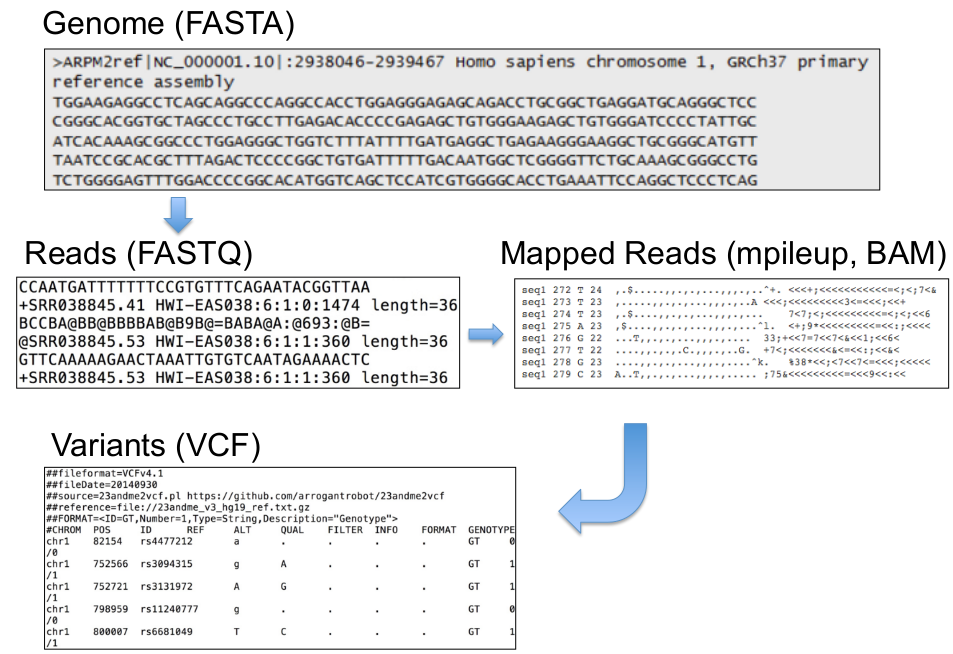
\includegraphics[width=\textwidth]{Pics/files.png}
	\end{figure}

}

%%%%%%%%%%%%%%%%%%%%%%%%%%%%%%%%%%%%%%%%%%%%%%%%

\begin{frame}
\frametitle{Our data: mapped reads with quality scores}

	\begin{figure}
                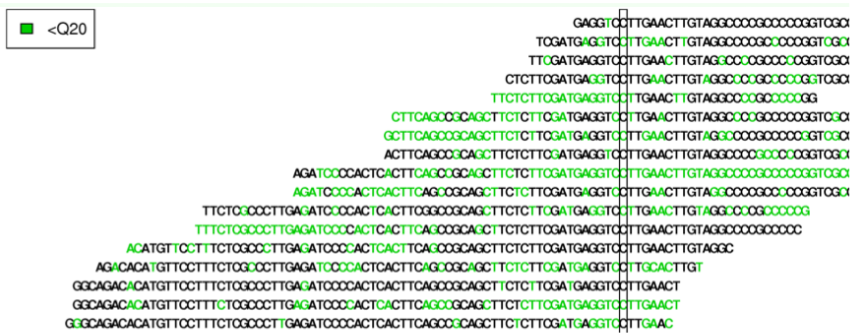
\includegraphics[width=\textwidth]{Pics/mapped_reads.png}
        \end{figure}

	\begin{itemize}
		\item Coverage:	fraction of the genome with data
		\item Depth: number of reads mapped to a position
		\item Counts: number of different alleles mapped to a position
		\item Effective Base Depth: similar to the counts, but weighing for qscores and mapping quality
	\end{itemize}

\end{frame}

%%%%%%%%%%%%%%%%%%%%%%%%%%%%%%%%%%%%%%%%%%%%%%%%%%

\frame{\frametitle{Challenges}

        \begin{figure}
                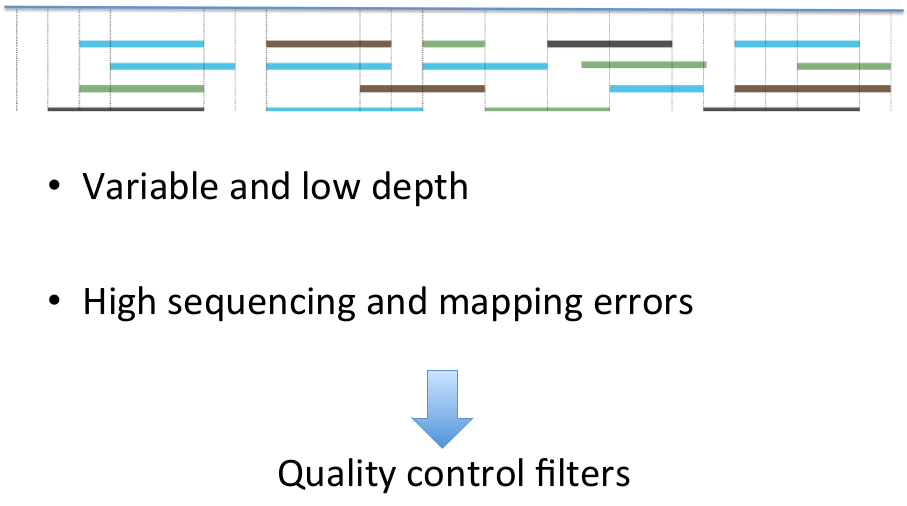
\includegraphics[width=\textwidth]{Pics/challenges.png}
        \end{figure}

}



% Genotype likelihoods

\section{Genotype likelihoods}

%%%%%%%%%%%%%%%%%%%%%%%%%%%%%%%%%%%%%%%%%%%%%%%%%
 
\frame{\frametitle{The data}

	\begin{figure}
		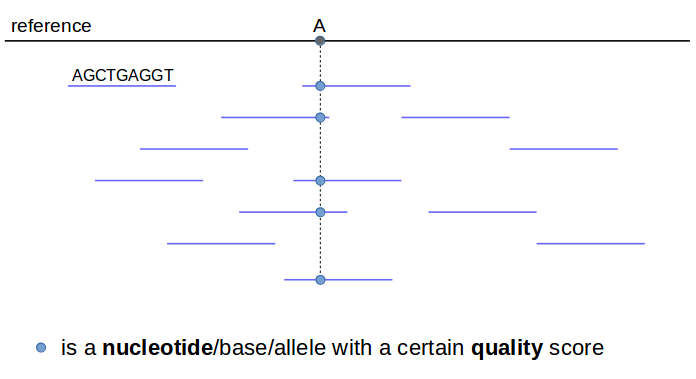
\includegraphics[scale=0.45]{Pics/mappedReads}
	\end{figure}

}

%%%%%%%%%%%%%%%%%%%%%%%%%%%%%%%%%%%%%%%%%%%%%%%%%%%%

\frame{\frametitle{Genotype likelihoods}

	\begin{block}{Likelihood}
		$P(D|G=\{A_1,A_2,...,A_n\})$
        \newline
		with
        \newline
		$A_i \in \{A,C,G,T\}$
        and $n$ being the ploidy
	\end{block}

How many genotypes likelihoods do we need to calculate for each each individual at each site?

}

%%%%%%%%%%%%%%%%%%%%%%%%%%%%%%%%%%%%%%%%%%%%%%%%%%%%

\frame{\frametitle{Genotype likelihoods}

	\begin{figure}
		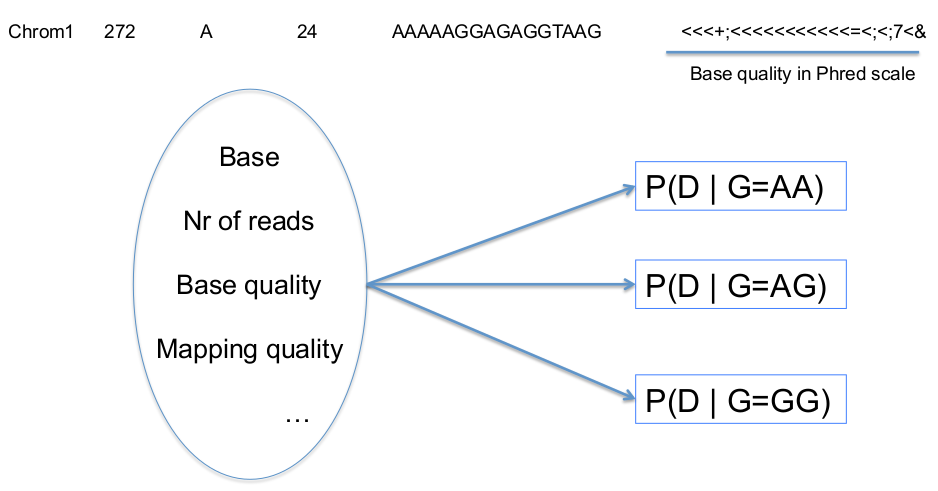
\includegraphics[scale=0.3]{Pics/genoLikes}
	\end{figure}

}


%%%%%%%%%%%%%%%%%%%%%%%%%%%%%%%%%%%%%%%%%%%%%%%%%%%%

\frame{\frametitle{Calculating genotype likelihoods}

\begin{block}{Likelihood function}

	\begin{equation*}
		P(D|G=\{A_1,A_2,...,A_N\}) = \prod_{i=1}^R \sum_{j=1}^N \frac{L_{A_j,i}}{N}
	\end{equation*}
 
 	\begin{itemize}
    	\item $L_{A_j,i} = P(D|A_G=A_j)$
    	\item $A_i \in \{A,C,G,T\}$
		\item $R$ is the depth (nr. of reads)
    	\item $N$ is the ploidy (nr. of chromosomes)
	\end{itemize}
    
\end{block}

Example: 
\newline
\footnotesize{A\\A\\A\\G\\}
with all quality scores equal to 20 (in phred score)
\newline
$P(D|G=AC) = ?$

}


%%%%%%%%%%%%%%%%%%%%%%%%%%%%%%%%%%%%%%%%%%%%%%%%%%%%

\frame{\frametitle{Calculating genotype likelihoods}

	\begin{block}{Likelihood function}

		\begin{equation*}
			P(D|G=\{A_1,A_2,...,A_N\}) = \prod_{i=1}^R \sum_{j=1}^N \frac{L_{A_j,i}}{N}
		\end{equation*}
  
	\end{block}

	\footnotesize{A\\A\\A\\G\\ \& Q=20}

	\begin{equation*}
		P(D|G=\{A,C\}) = ...
	\end{equation*}

}

%%%%%%%%%%%%%%%%%%%%%%%%%%%%%%%%%%%%%%%%%%%%%%%%%%%%%%%%%%%%%%%%%%%%

\frame{\frametitle{Calculating genotype likelihoods}

	\begin{block}{Likelihood function}

		\begin{equation*}
			P(D|G=\{A_1,A_2,...,A_N\}) = \prod_{i=1}^R \sum_{j=1}^N \frac{L_{A_j,i}}{N}
		\end{equation*}
  
	\end{block}

	\footnotesize{A\\A\\A\\G\\ \& Q=20}

	$N=2; i=1; A_1=A; A_2=C$

	\begin{equation*}
		P(D|G=\{A,C\}) = (\frac{L_{A,1}}{2} + \frac{L_{C,1}}{2}) \times ...
	\end{equation*}

	What are $L_{A,1}$ and $L_{C,1}$?

}

%%%%%%%%%%%%%%%%%%%%%%%%%%%%%%%%%%%%%%%%%%%%%%%%%%%%%%%%%%%%%%%%%%%%

\frame{\frametitle{Calculating genotype likelihoods}

	\begin{block}{Likelihood function}

		\begin{equation*}
			P(D|G=\{A_1,A_2,...,A_N\}) = \prod_{i=1}^R \sum_{j=1}^N \frac{L_{A_j,i}}{N}
		\end{equation*}
  
	\end{block}

	\footnotesize{A\\A\\A\\G\\ \& Q=20}

	\begin{equation*}
			L_{C,1} = \frac{\epsilon_1}{3}	
	\end{equation*}

	\begin{equation*}
	    	L_{A,1} = 1-\epsilon_1
	\end{equation*}
    
	\begin{equation*}
		P(D|G=\{A,C\}) = (\frac{1-\epsilon_1}{2} + \frac{\epsilon_1}{6}) \times ...
	\end{equation*}



}

%%%%%%%%%%%%%%%%%%%%%%%%%%%%%%%%%%%%%%%%%%%%%%%%%%%%%%%%%%%%%%%%%%%%

\frame{\frametitle{Calculating genotype likelihoods}

	\begin{block}{Likelihood function}

		\begin{equation*}
			P(D|G=\{A_1,A_2,...,A_N\}) = \prod_{i=1}^R \sum_{j=1}^N \frac{L_{A_j,i}}{N}
		\end{equation*}
  
	\end{block}

	\footnotesize{A\\A\\A\\G\\ \& Q=20}

	\begin{equation*}
			L_{C,1} = \frac{\epsilon_1}{3}	
	\end{equation*}

	\begin{equation*}
	    	L_{A,1} = 1-\epsilon_1
	\end{equation*}
    
	\begin{equation*}
		P(D|G=\{A,C\}) = (\frac{1-\epsilon_1}{2} + \frac{\epsilon_1}{6}) \times (\frac{1-\epsilon_2}{2} + \frac{\epsilon_2}{6}) \times (\frac{1-\epsilon_3}{2} + \frac{\epsilon_3}{6}) \times \frac{\epsilon_4}{3}
	\end{equation*}

	What are $\epsilon_1, \epsilon_2$, ...?

}

%%%%%%%%%%%%%%%%%%%%%%%%%%%%%%%%%%%%%%%%%%%%%%%%%%%%%%%%%%%%%%%%%%%%

\frame{\frametitle{Calculating genotype likelihoods}

	\begin{columns}
	
    	\column{0.6\textwidth}   

		\begin{center}
			\begin{tabular}{c | c}
			Genotype & Likelihood (log10)\\
    		\hline
	    	AA & -2.49\\
    		\textbf{AC} & \textbf{-3.38}\\
    		AG & -1.22\\
    		AT & -3.38\\
        	CC & -9.91\\
            CG & -7.74\\
            CT & -9.91\\
            GG & -7.44\\
            GT & -7.74\\
            TT & -9.91\\
        	\hline
			\end{tabular}
       	\end{center}

		\column{0.4\textwidth}

		\footnotesize{A\\A\\A\\G\\ \& $\epsilon=0.01$}

	\end{columns}

}



% Genotype calling

\section{Genotype calling, really?}

%%%%%%%%%%%%%%%%%%%%%%%%%%%%%%%%%%%%%%%%%%%%%%%%%%%

\frame{\frametitle{Genotype calling}

	\begin{columns}
	
    	\column{0.6\textwidth}   

		\begin{center}
			\begin{tabular}{c | c}
			Genotype & Likelihood (log10)\\
    		\hline
	    	AA & -2.49\\
    		AC & -3.38\\
    		AG & -1.22\\
    		AT & -3.38\\
            CC & -9.91\\
            CG & -7.74\\
            CT & -9.91\\
            GG & -7.44\\
            GT & -7.74\\
            TT & -9.91\\
        	\hline
			\end{tabular}
       	\end{center}

		\column{0.4\textwidth}

		AAAG \& $\epsilon=0.01$

		\begin{block}{}
			What is the genotype here?
		\end{block}

	\end{columns}


}

%%%%%%%%%%%%%%%%%%%%%%%%%%%%%%%%%%%%%%%%%%%%%%%%%%%

\frame{\frametitle{Genotype calling}

	\begin{columns}
	
    	\column{0.6\textwidth}   

		\begin{center}
			\begin{tabular}{c | c}
			Genotype & Likelihood (log10)\\
    		\hline
	    	AA & -2.49\\
    		AC & -3.38\\
    		\textbf{AG} & \textbf{-1.22}\\
    		AT & -3.38\\
            CC & -9.91\\
            CG & -7.74\\
            CT & -9.91\\
            GG & -7.44\\
            GT & -7.74\\
            TT & -9.91\\
        	\hline
			\end{tabular}
       	\end{center}

		\column{0.4\textwidth}

		AAAG \& $\epsilon=0.01$

		What is the genotype? AG.

		\begin{block}{Maximum Likelihood}
			The simplest genotype caller: choose the genotype with the highest likelihood.
		\end{block}

	\end{columns}


}

%%%%%%%%%%%%%%%%%%%%%%%%%%%%%%%%%%%%%%

\frame{\frametitle{Major and minor alleles}

	\begin{block}{Likelihood function}
		\begin{equation*}
			\log P(D|G=A) = \sum_{i=1}^R \log L_{A_j,i}
		\end{equation*}
	\end{block}

	AAAG \& $\epsilon=0.01$

	\begin{center}
		\begin{tabular}{c | c}
		Allele & log-Likelihood\\
    	\hline
	    \textbf{A} & \textbf{-2.49}\\
    	C & -3.38\\
    	\textbf{G} & \textbf{-1.22}\\
    	T & -3.38\\
        \hline
		\end{tabular}
	\end{center}

	We can reduce the genotype space to 3 entries (from 10).
    
}    
    
%%%%%%%%%%%%%%%%%%%%%%%%%%%%%%%%%%%%%%

\frame{\frametitle{Genotype likelihoods}

	AAAG \& `5555` \& A,G alleles

	\begin{center}
		\begin{tabular}{c | c}
		Genotype & log-Likelihood\\
    		\hline
	    	AA & -5.73\\
    		AG & -2.80\\
    		GG & -17.12\\
        	\hline
		\end{tabular}
	\end{center}

	Examples varying qualities and reads...
    
}   

%%%%%%%%%%%%%%%%%%%%%%%%%%%%%%%%%%%%%%%%%%%%%

\frame{\frametitle{Genotype likelihoods - example} 

        AAAG \& `555\textbf{0}` \& A,G alleles

        \begin{center}
                \begin{tabular}{c | c}
                Genotype & log-Likelihood\\
        	\hline
		\pause
            	AA & -4.58\\
        	AG & -2.81\\
        	GG & -17.14\\
        	\hline
          	\end{tabular}
        \end{center}

}

%%%%%%%%%%%%%%%%%%%%%%%%%%%%%%%%%%%%%%%%%%%%%

\frame{\frametitle{Genotype likelihoods - example}

        AAAG \& `555\textbf{K}` \& A,G alleles

        \begin{center}
                \begin{tabular}{c | c}
                Genotype & log-Likelihood\\
                \hline
                \pause
                AA & -10.80\\
                AG & -2.80\\
                GG & -17.11\\
                \hline
                \end{tabular}
        \end{center}

}

%%%%%%%%%%%%%%%%%%%%%%%%%%%%%%%%%%%%%%%%%%%%%

\frame{\frametitle{Genotype likelihoods - example}

        AAAAAAAAAG \& `5555555550` \& A,G alleles

        \begin{center}
                \begin{tabular}{c | c}
                Genotype & log-Likelihood\\
                \hline
                \pause
                AA & -4.64\\
                AG & -7.01\\
                GG & -51.37\\
                \hline
                \end{tabular}
        \end{center}

}

%%%%%%%%%%%%%%%%%%%%%%%%%%%%%%%%%%%

\begin{frame}
\frametitle{NGS data uncertainty}

	\begin{block}{Issue}
		There is a notable amount of statistical uncertainty in assigning individual genotypes depending on the number of reads and their quality.
		How can we deal with that when doing population genetics analysis (e.g. estimating genetic diversity)?
	\end{block}

	\begin{block}{Solutions}
		\begin{enumerate}
			\item let's pretend we don't have such uncertainty
			\pause
			\item genotype filtering
			\item (a third way)
		\end{enumerate}
	\end{block}

\end{frame}

%%%%%%%%%%%%%%%%%%%%%%%%%%%%%%%%%%%%%%%%%%%

\frame{\frametitle{Genotype likelihood ratio}

	\begin{equation*}
		\log_{10} \frac{L_{G(1)}}{L_{G(2)}} > t
	\end{equation*}

	i.e. $t=1$ meaning that the most likely genotype is 10 times more likely than the second most likely one

}

%%%%%%%%%%%%%%%%%%%%%%%%%%%%%%%%%%%%%%%%%%%%%%%%%%%%

\frame{
\frametitle{Genotype posterior probability}

	AAAG \& $\epsilon=0.01$ \& A,G alleles

	\begin{center}
		\begin{tabular}{c | c | c | c}
		Genotype & Likelihood (log) & Prior & Posterior\\
    	\hline
	    AA & -5.73 & 1/3 & 0.05\\
    	AG & -2.80 & 1/3 & 0.95\\
    	GG & -17.12 & 1/3 & ~0\\
        \hline
		\end{tabular}
	\end{center}

	Only call genotypes if the largest probability is above a certain threshold (e.g. 0.95).

	\begin{center}
                Pros and cons?
                \pause
                \begin{itemize}
                \item Yes: genotype are called with higher \textbf{confidence}
                \item No: more \textbf{missing} data
                \end{itemize}
        \end{center}



}

%%%%%%%%%%%%%%%%%%%%%%%%%%%%%%%%%%%%%%%%%%%%%%%%%

\begin{frame}
\frametitle{Exercise 1}

	Simulate NGS data and calculate genotype likelihoods and probabilities.

	Assess the amount of uncertainty and data missingness.

\end{frame}





\subsection{Low-depth (uknown genotypes)}

\begin{frame}
\frametitle{NGS data processing in the \textbf{model} world}

	\begin{figure}
		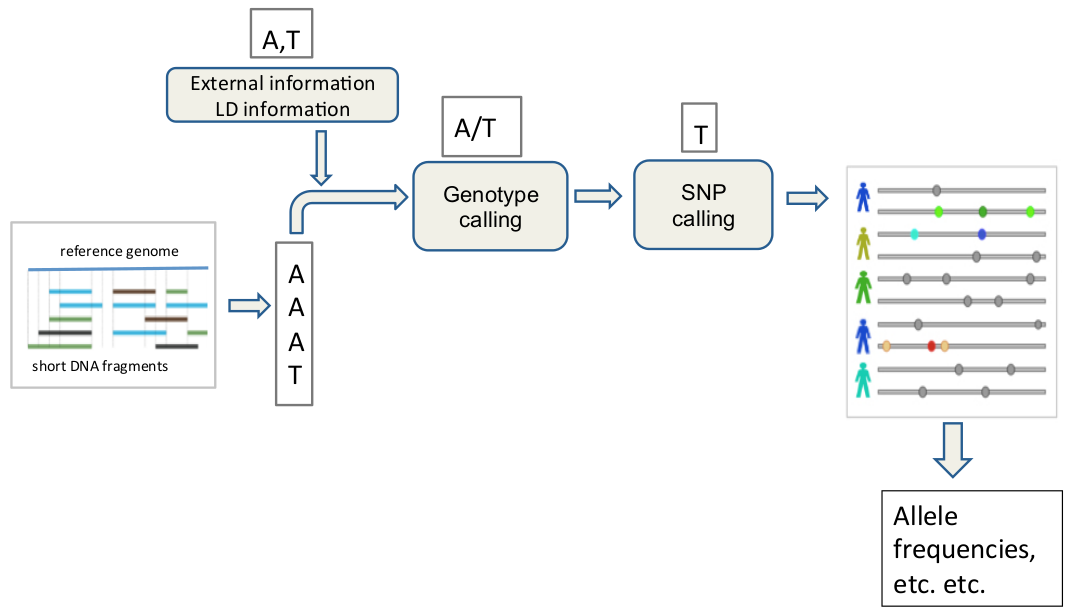
\includegraphics[width=\textwidth]{Pics/ngs_1.png}
	\end{figure}

\end{frame}

\begin{frame}
\frametitle{NGS data processing in the \textbf{non-model} world}

	\begin{figure}
        	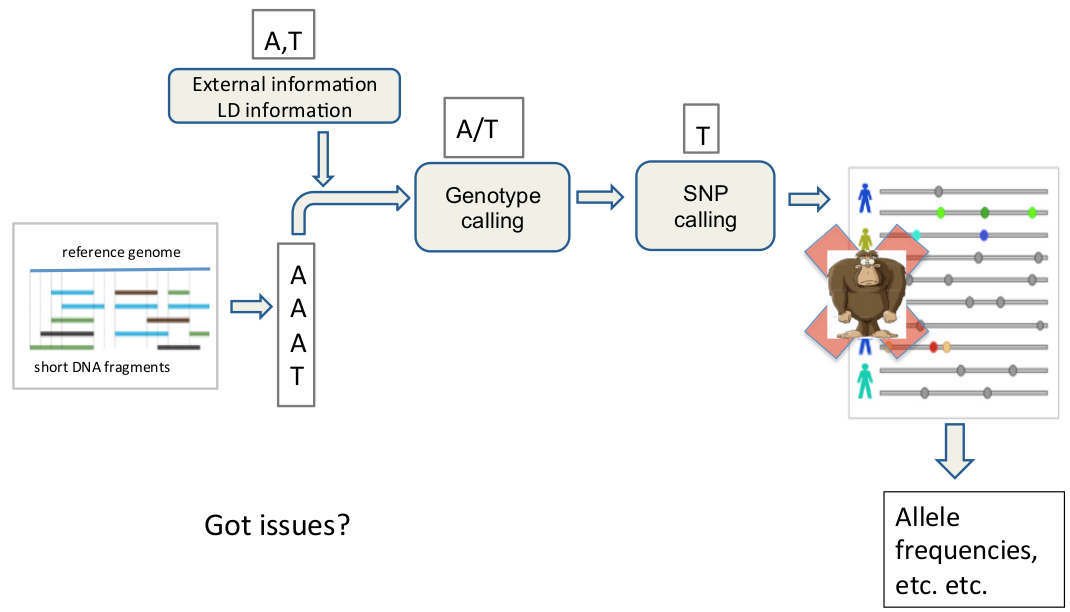
\includegraphics[width=\textwidth]{Pics/ngs_2.png}
	\end{figure}

\end{frame}

\begin{frame}
\frametitle{NGS data processing in the \textbf{non-model} world}

	\begin{figure}
        	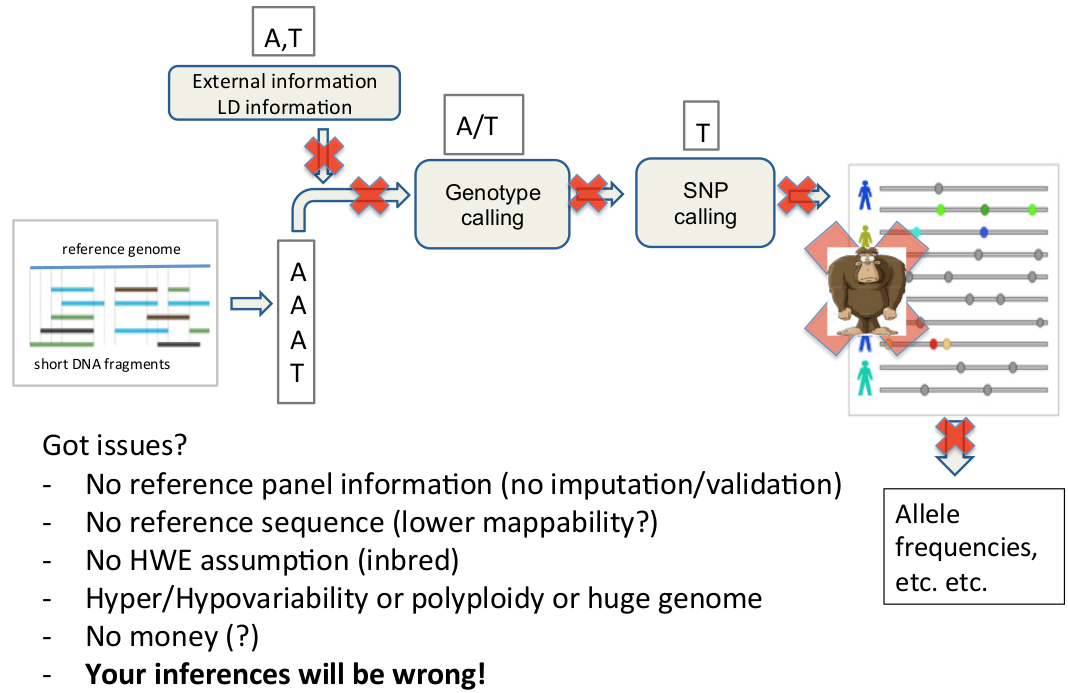
\includegraphics[width=\textwidth]{Pics/ngs_3.png}
	\end{figure}

\end{frame}

\begin{frame}
\frametitle{NGS data processing in the \textbf{non-model} world}

	\begin{figure}
        	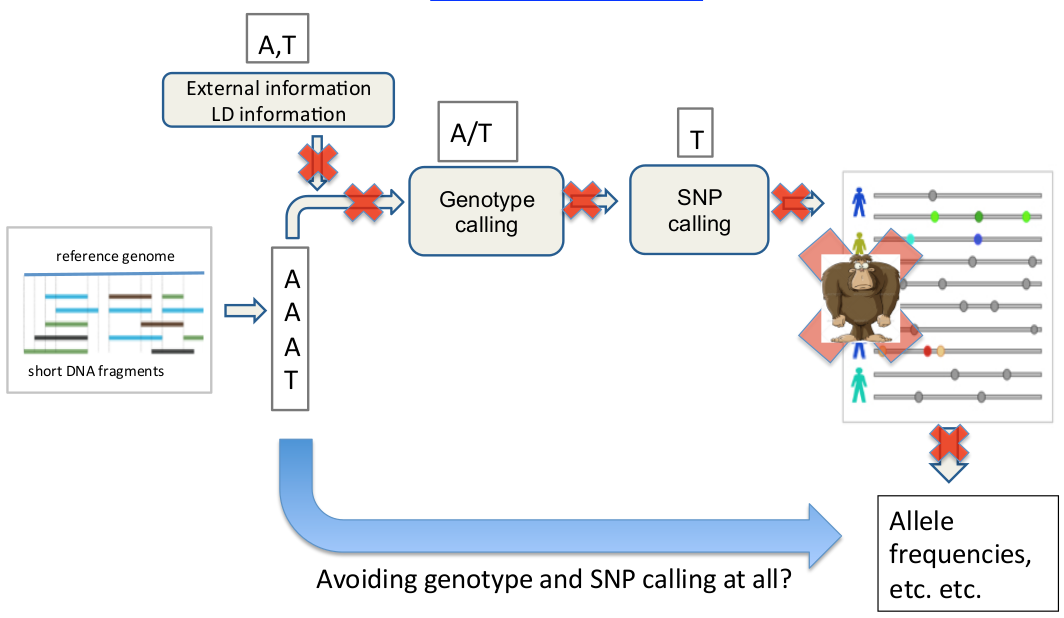
\includegraphics[width=\textwidth]{Pics/ngs_4.png}
	\end{figure}

\end{frame}


%%%%%%%%%%%%%%%%%%%%%%%%%%%%%%%%%%%%%%%%%%%%%%

\begin{frame}
\frametitle{Summary statistics}

	Aim: estimate the number of heterozygotes ($H$) from \textbf{unknown} genotypes.

	Data:
	\begin{center}
                \begin{tabular}{c | c | c | c | c}
                	Sample & Data & $P(G=AA|D)$ & $P(G=AG|D)$ & $P(G=GG|D)$\\
        		\hline
			1 & A & 0.66 & 0.33 & 0.01\\
			2 & AAAG & 0.14 & 0.86 & 0.00\\
			3 & AGG & 0.00 & 0.92 & 0.08\\
			4 & GG & 0.00 & 0.20 & 0.80\\
        		\hline
                \end{tabular}
		with $Q=15$
        \end{center}

	Solutions:
	\begin{enumerate}
		\item call genotypes: $H=2$
		\pause
		\item sample genotypes: $H$ is defined by a distribution 
	\end{enumerate}


\end{frame}

%%%%%%%%%%%%%%%%%%%%%%%%%%%%%%%%%%%%%%%%%%%

\begin{frame}
\frametitle{Summary statistics}

	\tiny{
        \begin{center}
                \begin{tabular}{c | c | c | c | c}
                        Sample & Data & $P(G=AA|D)$ & $P(G=AG|D)$ & $P(G=GG|D)$\\
                        \hline
                        1 & A & 0.66 & 0.33 & 0.01\\
                        2 & AAAG & 0.14 & 0.86 & 0.00\\
                        3 & AGG & 0.00 & 0.92 & 0.08\\
                        4 & GG & 0.00 & 0.20 & 0.80\\
                        \hline
                \end{tabular}
                with $Q=15$
        \end{center}
	}
	
	Sampling genotypes:
	\begin{figure}
		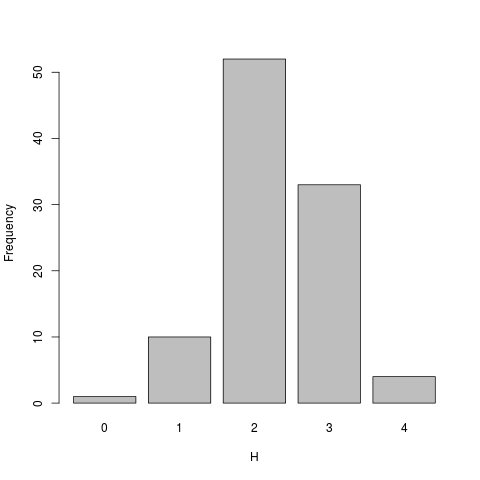
\includegraphics[width=0.45\textwidth]{Pics/H.png}
	\end{figure}


\end{frame}

%%%%%%%%%%%%%%%%%%%%%%%%%%%%%%%%%%%%%%%%%%%%

\begin{frame}
\frametitle{Expected value}

	\begin{figure}
                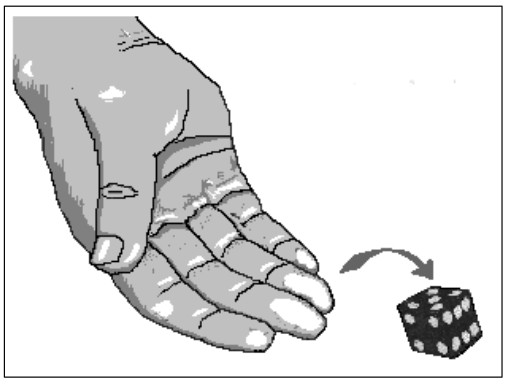
\includegraphics[width=0.5\textwidth]{Pics/die.png}
        \end{figure}

	\begin{itemize}
		\item What are the possible outcomes of this experiment?
		\item With what probability?
	\end{itemize}

\end{frame}

%%%%%%%%%%%%%%%%%%%%%%%%%%%%%%%%%%%%%%%%%%%%

\begin{frame}
\frametitle{Expected value}

	The expected	value	of	a	discrete	random	variable	is	the probability-weighted	average	of	all	possible	values

	\begin{equation*}
		E[X|D] = \sum_{i=1}^N x_i p(X=x_i|D)
	\end{equation*}
	
	\pause

	
		$E[X|D] = 1 \cdot \frac{1}{6} + 2 \cdot \frac{1}{6} + 3 \cdot \frac{1}{6} + 4 \cdot \frac{1}{6} + 5 \cdot \frac{1}{6} +6 \cdot \frac{1}{6} = \frac{(1+2+3+4+5+6)}{6} = \frac{21}{6} = 3.5$

\end{frame}

%%%%%%%%%%%%%%%%%%%%%%%%%%%%%%%%

\begin{frame}
\frametitle{Expected value}

		It is the average value if you perform the same experiment many times.

        	\begin{figure}
                	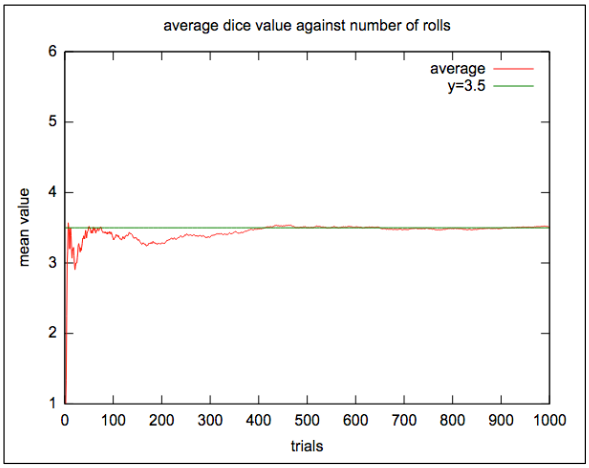
\includegraphics[width=0.5\textwidth]{Pics/die_tries.png}
        	\end{figure}

\end{frame}

%%%%%%%%%%%%%%%%%%%%%%%%%%%%%%%%%%%%%%%%%%%%

\begin{frame}
\frametitle{Summary statistics}

        \tiny{
        \begin{center}
                \begin{tabular}{c | c | c | c | c}
                        Sample & Data & $P(G=AA|D)$ & $P(G=AG|D)$ & $P(G=GG|D)$\\
                        \hline
                        1 & A & 0.66 & 0.33 & 0.01\\
                        2 & AAAG & 0.14 & 0.86 & 0.00\\
                        3 & AGG & 0.00 & 0.92 & 0.08\\
                        4 & GG & 0.00 & 0.20 & 0.80\\
                        \hline
                \end{tabular}
                with $Q=15$
        \end{center}
        }

	\large{
	\begin{enumerate}
                \item call genotypes: $H=2$
                \item sample genotypes: $H$ is defined by a distribution
		\item expected value: $\hat{H}$ = \pause $p(G_1=AG) + p(G_2=AG) + p(G_3=AG) + p(G_4=AG) = 0.33+0.86+0.92+0.20 = 2.31$
        \end{enumerate}
	}

\end{frame}


%%%%%%%%%%%%%%%%%%%%%%%%%%%%%%%%%%%%%%%%%%%%%%%

\begin{frame}
\frametitle{Genetic distances}

	\begin{figure}
                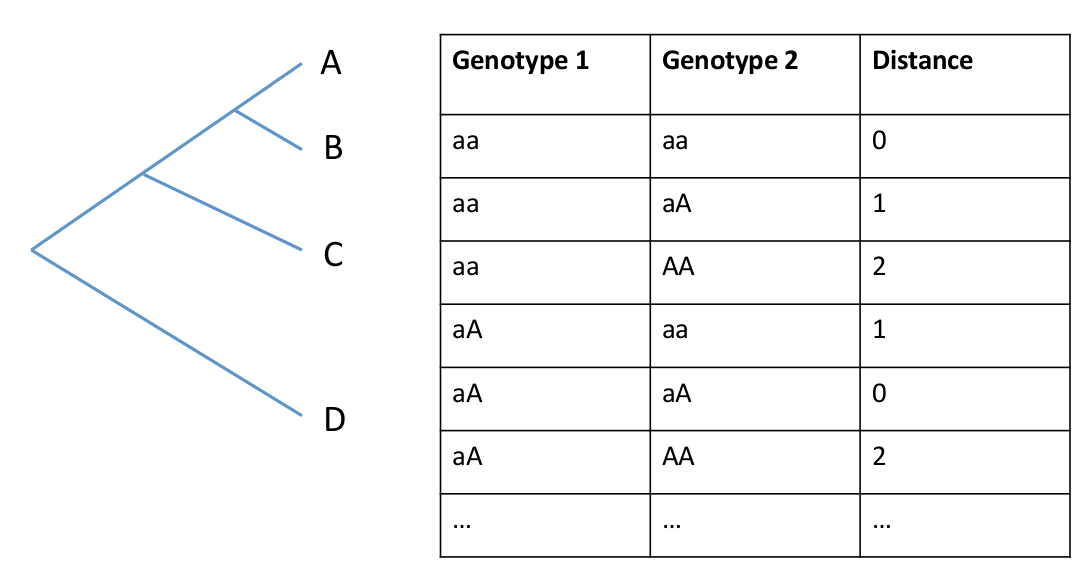
\includegraphics[width=\textwidth]{Pics/gdist_1.png}
        \end{figure}


\end{frame}

%%%%%%%%%%%%%%%%%%%%%%%%%%%%%%%%%%%%%%%%%%%%%%%

\begin{frame}
\frametitle{Genetic distances}

        \begin{figure}
                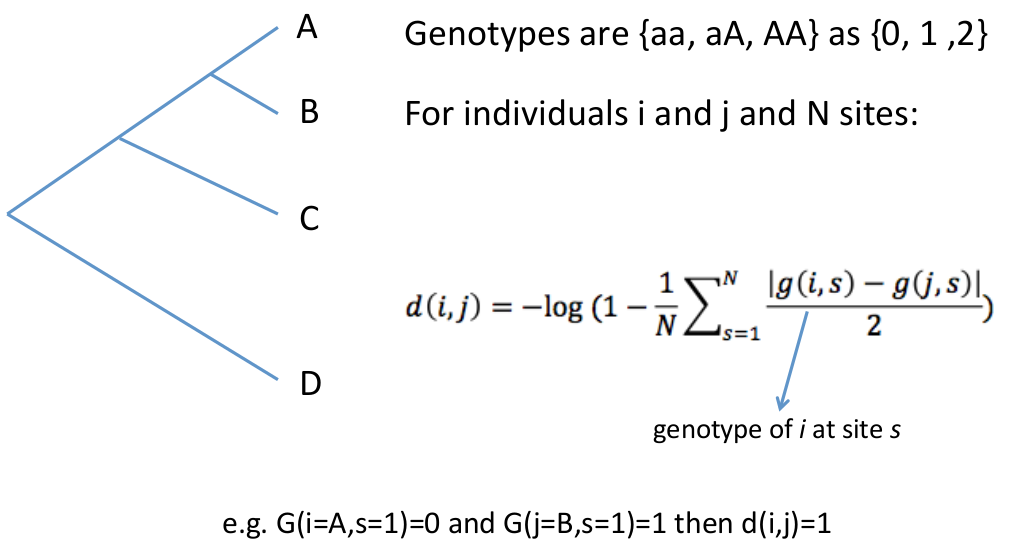
\includegraphics[width=\textwidth]{Pics/gdist_2.png}
        \end{figure}

\end{frame}

%%%%%%%%%%%%%%%%%%%%%%%%%%%%%%%%%%%%%%%%%%%%%%%

\begin{frame}
\frametitle{Genetic distances from known genotypes}

        \begin{figure}
                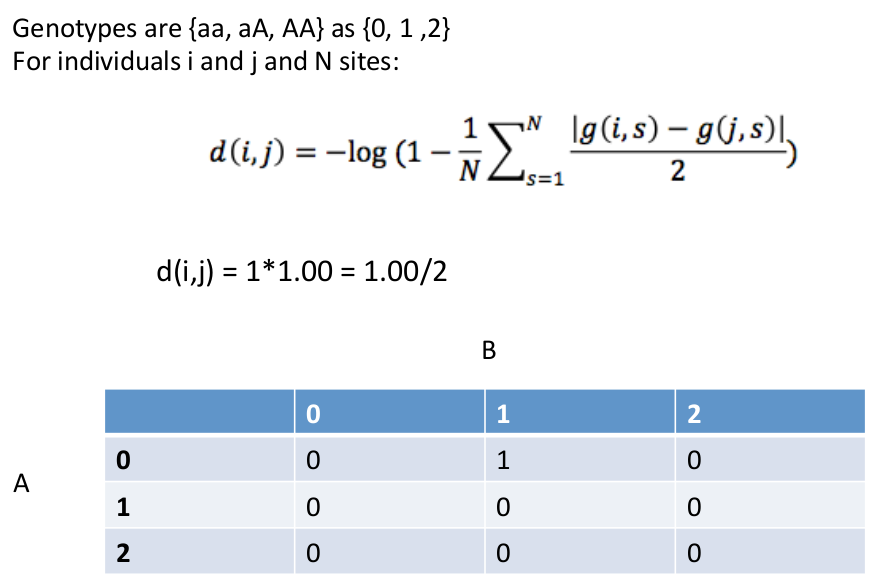
\includegraphics[width=\textwidth]{Pics/gdist_3.png}
        \end{figure}

\end{frame}

%%%%%%%%%%%%%%%%%%%%%%%%%%%%%%%%%%%%%%%%%%%%%%%

\begin{frame}
\frametitle{Genetic distances from \textbf{unknown} genotypes}

        \begin{figure}
                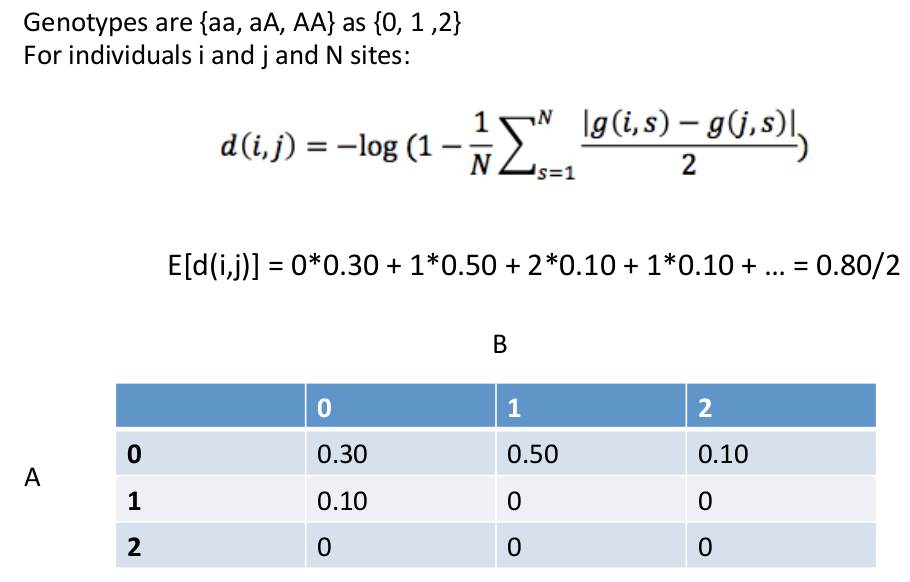
\includegraphics[width=\textwidth]{Pics/gdist_4.png}
        \end{figure}

\end{frame}

%%%%%%%%%%%%%%%%%%%%%%%%%%%%%%%%%%%%%%%%%%%%%%%

\begin{frame}
\frametitle{Genetic distances from \textbf{unknown} genotypes}

        \begin{figure}
                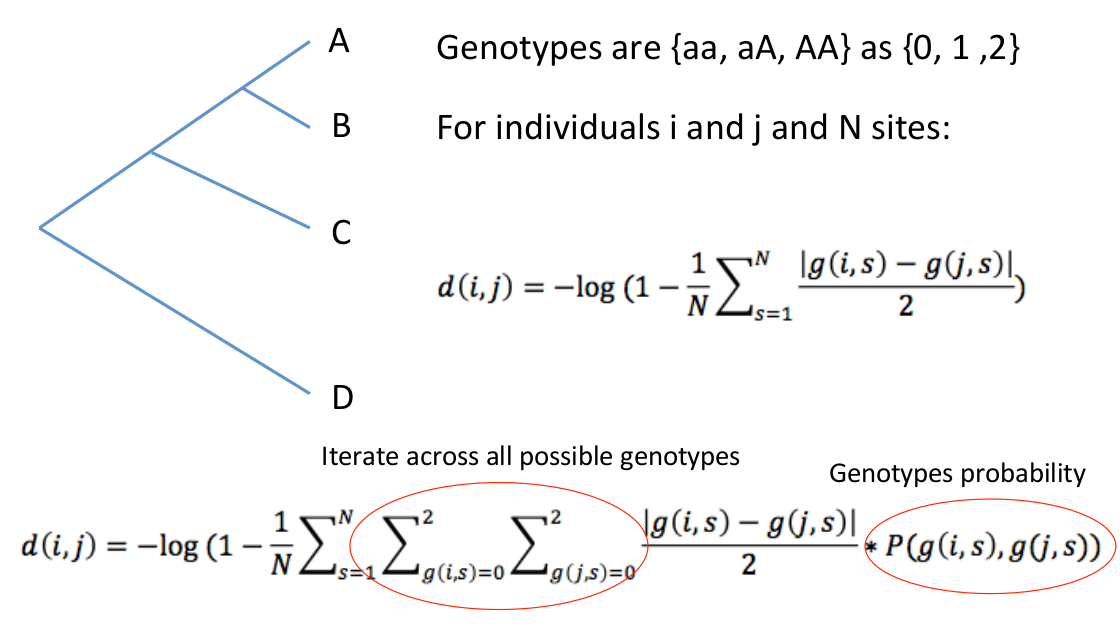
\includegraphics[width=\textwidth]{Pics/gdist_5.png}
        \end{figure}

\end{frame}

%%%%%%%%%%%%%%%%%%%%%%%%%%%%%%%%%%%%%%%%%%%%%%%

\begin{frame}
\frametitle{Genetic distances from \textbf{unknown} genotypes}

        \begin{figure}
                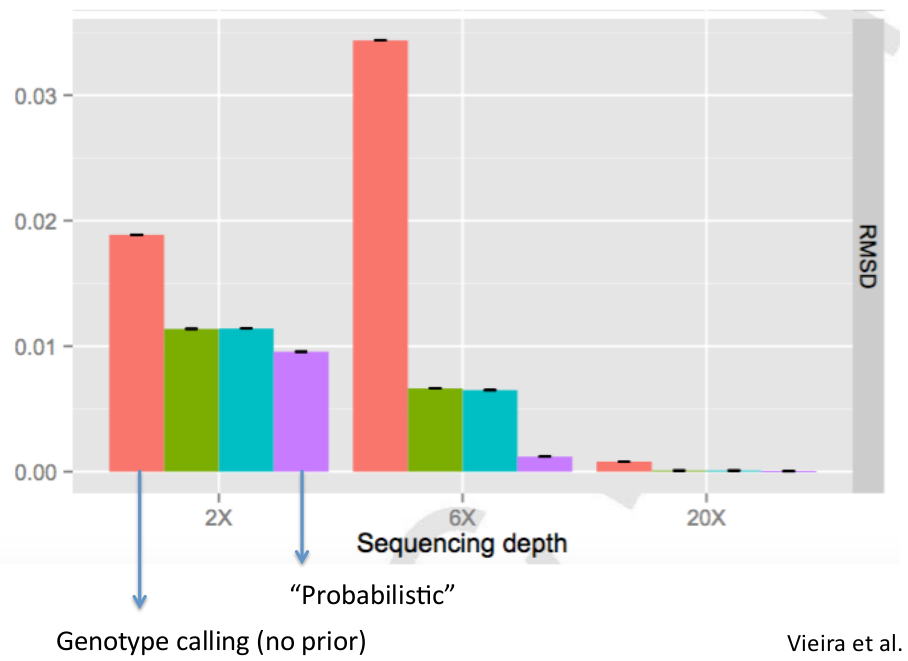
\includegraphics[width=\textwidth]{Pics/gdist_6.png}
        \end{figure}

\end{frame}

%%%%%%%%%%%%%%%%%%%%%%%%%%%%%%%%%%%%%%%%%%%%%%%

\begin{frame}
\frametitle{Clustering from \textbf{unknown} genotypes}

        \begin{figure}
                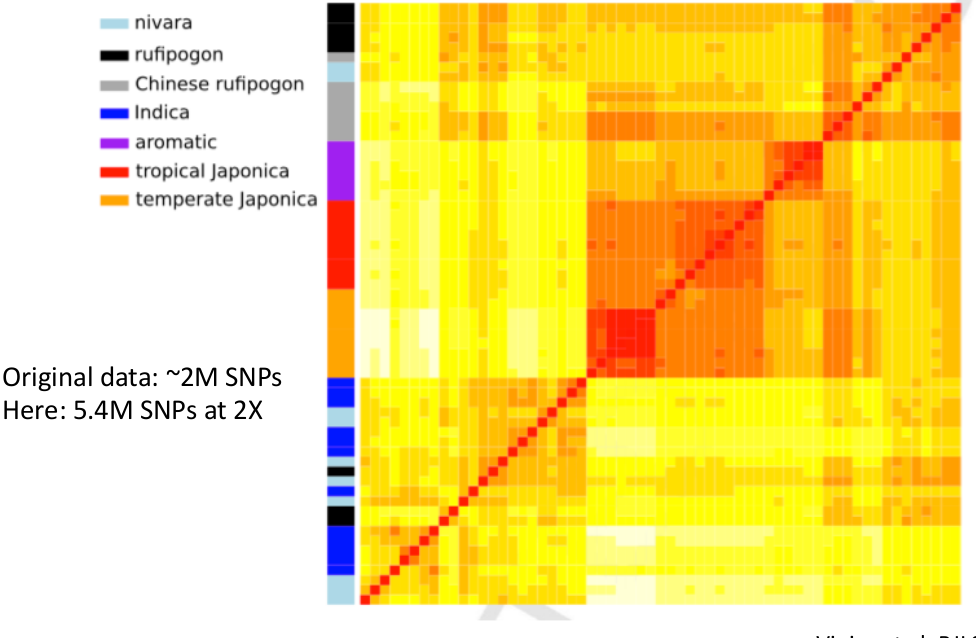
\includegraphics[width=\textwidth]{Pics/gdist_7.png}
        \end{figure}

\end{frame}


%%%%%%%%%%%%%%%%%%%%%%%%%%%%%%%%%%%%%%%%%%%%%

\begin{frame}
\frametitle{Population structure}

	Principal Compoment Analysis (PCA) is a data reduction method for:
	\begin{itemize}
		\item visualisation
		\item correction for population stratification
		\item information on population history and differentiation?
	\end{itemize}

	\begin{figure}
                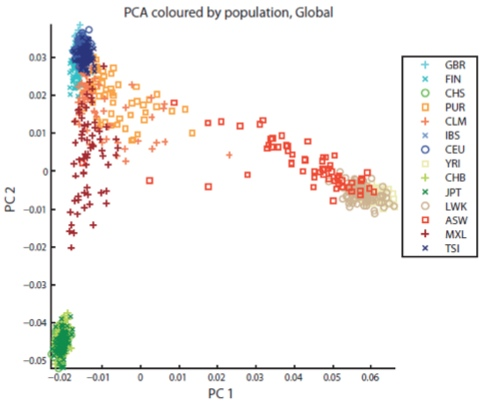
\includegraphics[width=0.5\textwidth]{Pics/pca.jpg}
        \end{figure}

\end{frame}

%%%%%%%%%%%%%%%%%%%%%%%%%%%%%%%%%%%%%%%%%%%%%%

\begin{frame}
\frametitle{Covariance matrix}

	\begin{figure}
                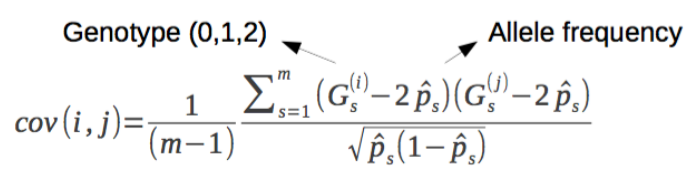
\includegraphics[width=0.70\textwidth]{Pics/covar.png}
        \end{figure}

	\pause

	\begin{figure}
                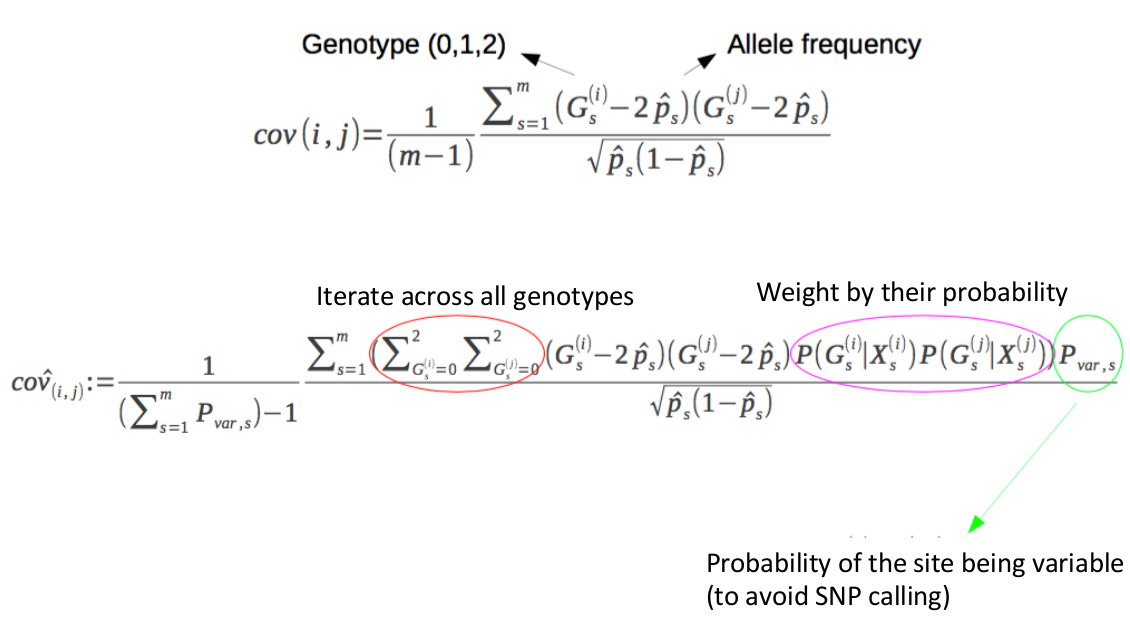
\includegraphics[width=0.70\textwidth]{Pics/covar_ngs.png}
        \end{figure}

	\footnotesize{Does it really work?}

\end{frame}


%%%%%%%%%%%%%%%%%%%%%%%%%%%%%%%%%%%%%%%%%%%%%%%

\begin{frame}
\frametitle{Exercise 2}

	Perform a PCA with called genotypes and using genotype probabilities. 
	
	Assess their relative performance.

\end{frame}









% Allele frequencies and SNP calling

\section{Allele frequencies}

%%%%%%%%%%%%%%%%%%%%%%%%%%%%%%%%%%%%%%%%%%%%%%%%%%%%%%%%%%

\frame{
\frametitle{Estimating allele frequencies}

	Assuming 2 alleles (A,G) with true allele frequency of 0.50

	\begin{center}
	\begin{tabular}{c|c|c|c}
	Sample & True genotype & Reads allele A & Read allele G\\
    \hline
    1 & AA & 7 & 0\\
    2 & AA & 25 & 1\\
    3 & AG & 5 & 3\\
    4 & AG & 4 & 4\\
    5 & GG & 0 & 2\\
    6 & GG & 0 & 4\\
    \hline
	\end{tabular}	
	\end{center}

	What is the simplest estimator of allele frequencies?

}


%%%%%%%%%%%%%%%%%%%%%%%%%%%%%%%%%%%%%%%%%%%%%%%%%%%%%%%%%%

\frame{
\frametitle{Estimating allele frequencies}

	Assuming 2 alleles (A,G) with true allele frequency of 0.50

	\begin{center}
	\begin{tabular}{c|c|c|c}
	Sample & True genotype & Reads allele A & Read allele G\\
    \hline
    1 & AA & 7 & 0\\
    2 & AA & 25 & 1\\
    3 & AG & 5 & 3\\
    4 & AG & 4 & 4\\
    5 & GG & 0 & 2\\
    6 & GG & 0 & 4\\
    \hline
    Total & & 41 & 14\\
    \hline
	\end{tabular}
	\end{center}

	\begin{equation*}
		\hat{f} = \frac{\sum_{i=1}^N n_{A,i}}{ \sum_{i=1}^N (n_{A,i}+n_{G,i}) }
	\end{equation*}

	$\hat{f}=0.75$

	What is wrong with this estimator?

}

%%%%%%%%%%%%%%%%%%%%%%%%%%%%%%%%%%%%%%%%%%%%%%%%%%%%%%%%%%

\frame{
\frametitle{Estimating allele frequencies}

	Assuming 2 alleles (A,G) with true allele frequency of 0.50

	\begin{center}
	\begin{tabular}{c|c|c|c}
	Sample & True genotype & Reads allele A & Read allele G\\
    \hline
    1 & AA & 7 & 0\\
    2 & AA & 25 & 1\\
    3 & AG & 5 & 3\\
    4 & AG & 4 & 4\\
    5 & GG & 0 & 2\\
    6 & GG & 0 & 4\\
    \hline
    Total & & 41 & 14\\
    \hline
	\end{tabular}
	\end{center}
    
    	\begin{equation*}
		\hat{n_A} = \sum_{i=1}^N (1-\epsilon)n_{A,i} + \epsilon n_{G,i} - \epsilon n_{A,i} - (1-\epsilon)n_{G,i}
	\end{equation*}
	
	%\begin{equation*}
	%	\hat{n_A}=\sum_{i=1}^N (1-\epsilon)(n_{A,i}-n_{G,i}) + \epsilon(n_{G,i}-n_{A,i})
	%\end{equation*}
    
    $\hat{f}=0.77$
}


%%%%%%%%%%%%%%%%%%%%%%%%%%%%%%%%%%%%%%%%%%%%%%%%%%%%%%%%%%

\frame{
\frametitle{Estimating allele frequencies}

	\begin{block}{Maximum Likelihood estimator}
		\begin{equation*}
			P(D|f) = \prod_{i=1}^N \sum_{g \in \{0,1,2\}} P(D|G=g) P(G=g|f)
		\end{equation*}
	\end{block}

}

%%%%%%%%%%%%%%%%%%%%%%%%%%%%%%%%%%%%%%%%%%%%%%%%%%%%%%%%%%

\frame{
\frametitle{Estimating allele frequencies}

        \begin{block}{Maximum Likelihood estimator}
                \begin{equation*}
                        P(D|f) = \prod_{i=1}^N \sum_{g \in \{0,1,2\}} P(D|G=g) P(G=g|f)
                \end{equation*}
        \end{block}

        $P(D|G=g)$ is the genotype likelihood and $P(G=g|f)$ is given by HWE (for instance).

	\begin{center}
        In our previous example, $\hat{f}=0.46$ which is much closer to the true value than previous estimators.
	\end{center}

}

%%%%%%%%%%%%%%%%%%%%%%%%%%%%%%%%%%%%%%%%%%%%%%%%%%%%%%%%%%%%%

\frame{
\frametitle{SNP calling}

	\begin{block}{Challenges}
	\begin{itemize}
	\item If high levels of missing data, then genotypes can be lost.
    \item Rare variants are hard to detect.
    \item Trade off between false positive and false negative rates.
	\end{itemize}
	\end{block}

	\begin{block}{How to call SNPs?}
	\begin{itemize}
	\item If at least one heterozygous genotype has been called.
    \item If the estimated allele frequency is above a certain threshold.
	\end{itemize}
	\end{block}

	Call a SNP if
	\begin{equation*}
        	\hat{f} \geq t
	\end{equation*}
	where $t$ can be the minimum sample allele frequency detectable (e.g. $t=1/2N$ with $N$ diploids).

}

%%%%%%%%%%%%%%%%%%%%%%%%%%%%%%%%%%%%%%%%%%%%%%%%%%%%%%%%%%%%%

\frame{
\frametitle{Likelihood Ratio Test}

A Likelihood Ratio Test (LRT) compares the goodness	of fit between the null and the alternative model:
\begin{itemize}
\item Null model: $f=0$
\item Alternative model: $f \neq 0$
\end{itemize}

\begin{equation*}
T = -2 \log \frac{L(f=0)}{L(f=\hat{f}_{MLE})}
\end{equation*}

where $T$ is $\chi^2$ distributed with 1 degree of freedom.

}

%%%%%%%%%%%%%%%%%%%%%%%%%%%%%%%%%%%%%%%%%%%%%%%%%

\begin{frame}
\frametitle{Exercise 3}

	Estimate allele frequencies and call SNPs.

	Assess the accuracy using different thresholds.

	Perform a new PCA with data filtering.

\end{frame}







\subsection{Low-depth (allele frequencies)}

%%%%%%%%%%%%%%%%%%%%%%%%%%%%%%%%%%%%%%%%%

\begin{frame}
\frametitle{Sample allele frequency likelihoods}

        \begin{equation*}
                        P(D|f) = \prod_{i=1}^N \sum_{g \in \{0,1,2\}} P(D|G=g) P(G=g|f)
        \end{equation*}

	\begin{center}
                \begin{tabular}{| c | c | c | c | c |}
			\hline
			$P(D|f=0)$ & $P(D|f=1)$ & $P(D|f=2)$ & ... & $P(D|f=2k)$\\
			\hline
                \end{tabular}
                with $k$ diploids.
        \end{center}

\end{frame}

%%%%%%%%%%%%%%%%%%%%%%%%%%%%%%%%%%%%%%%%%%

\begin{frame}
\frametitle{Sample allele frequency probabilities}

	\begin{figure}
                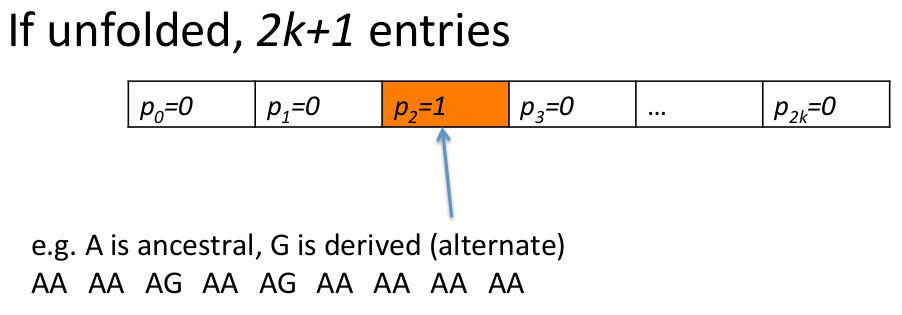
\includegraphics[width=\textwidth]{Pics/saf_1.png}
        \end{figure}
	
	If genotypes are unknown and counting is not possible?

\end{frame}

%%%%%%%%%%%%%%%%%%%%%%%%%%%%%%%%%%%%%%%%%%

\begin{frame}
\frametitle{Sample allele frequency probabilities}

        \begin{figure}
                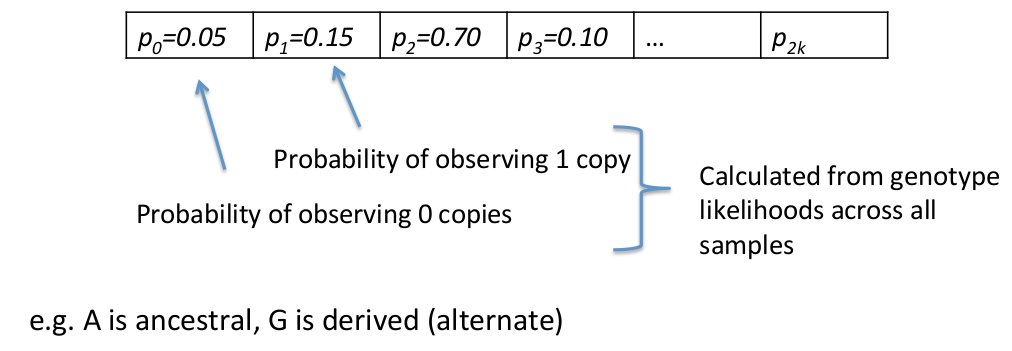
\includegraphics[width=\textwidth]{Pics/saf_2.png}
        \end{figure}

        If genotypes are unknown and counting is not possible.

\end{frame}

%%%%%%%%%%%%%%%%%%%%%%%%%%%%%%%%%%%%%%%

\begin{frame}
\frametitle{Sample allele frequency probabilities}

        \begin{figure}
                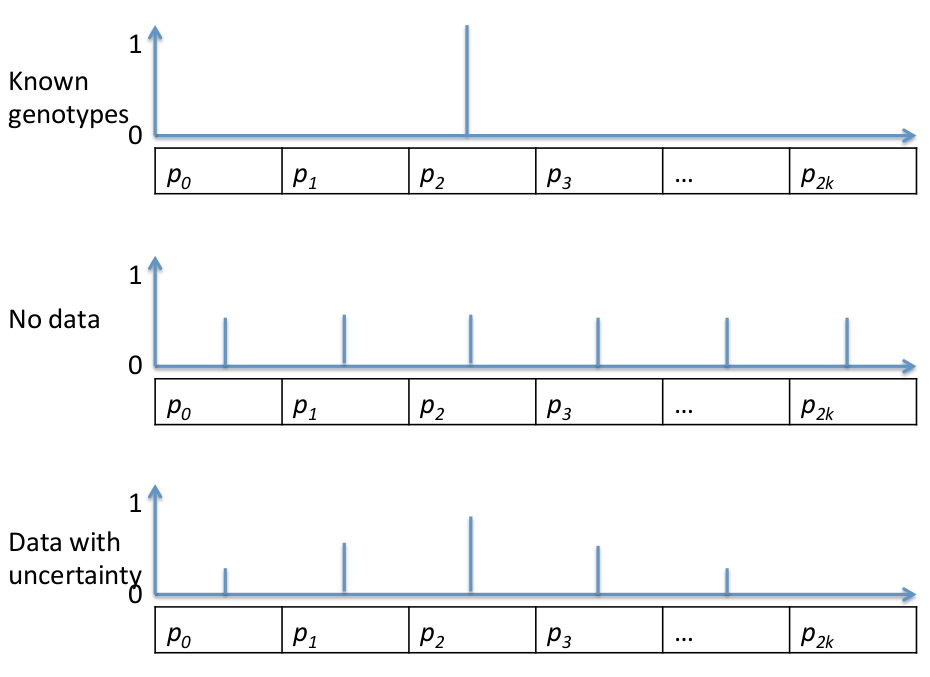
\includegraphics[width=0.7\textwidth]{Pics/saf_3.png}
        \end{figure} 

\end{frame}


%%%%%%%%%%%%%%%%%%%%%%%%%%%%%%%%%%

\begin{frame}
\frametitle{Sample allele frequency probabilities}

	Summary statistics

	\small{
	\begin{center}
                \begin{tabular}{| c | c | c | c | c |}
                        \hline
                        $P(f=0|D)$ & $P(f=1|D)$ & $P(f=2|D)$ & ... & $P(f=2k|D)$\\
                        \hline
                \end{tabular}\\
                with $k$ diploids.
        \end{center}
	}

	\begin{center}
		\Large{
		$\hat{f} = \pause \sum_{i=0}^{2k} (\frac{i}{2k}) \cdot P(f=i|D) $
		}
	\end{center}

\end{frame}

%%%%%%%%%%%%%%%%%%%%%%%%%%%%%%%%

\begin{frame}
\frametitle{Sample allele frequency probabilities}

        Summary statistics

        \small{
        \begin{center}
                \begin{tabular}{| c | c | c | c | c |}
                        \hline
                        $P(f=0|D)$ & $P(f=1|D)$ & $P(f=2|D)$ & ... & $P(f=2k|D)$\\
                        \hline
                \end{tabular}\\
                with $k$ diploids.
        \end{center}
        }

        \begin{center}
                \Large{
                $P_{\textit{var}} = \pause 1 - P(f=0|D) - P(f=2k|D) $
                }
        \end{center}

\end{frame}


%%%%%%%%%%%%%%%%%%%%%%%%%%%%%%%%

\begin{frame}
\frametitle{Sample allele frequency probabilities}

        Summary statistics - number of segregating sites

        \small{
        \begin{center}
                \begin{tabular}{| c | c | c | c | c | c |}
                        \hline
                        site 1 & $P(f=0|D)$ & $P(f=1|D)$ & $P(f=2|D)$ & ... & $P(f=2k|D)$\\
			site 2 & $P(f=0|D)$ & $P(f=1|D)$ & $P(f=2|D)$ & ... & $P(f=2k|D)$\\
			site 3 & $P(f=0|D)$ & $P(f=1|D)$ & $P(f=2|D)$ & ... & $P(f=2k|D)$\\
			... & ... & ... & ... & ...\\
			site M & $P(f=0|D)$ & $P(f=1|D)$ & $P(f=2|D)$ & ... & $P(f=2k|D)$\\
                        \hline
                \end{tabular}
        \end{center}
        }

        \begin{center}
                \Large{
                $E[S] = \pause \sum_{j=1}^M \pause (1 - P(f_j=0|D) - P(f_j=2k|D)) $   
                }
        \end{center}

\end{frame}

%%%%%%%%%%%%%%%%%%%%%%%%%%%%%%%%

\begin{frame}
\frametitle{Sample allele frequency probabilities}

        Summary statistics - nucleotide diversity $D=2 \cdot f \cdot (1-f)$

        \small{
        \begin{center} 
                \begin{tabular}{| c | c | c | c | c | c |}
                        \hline
                        site 1 & $P(f=0|D)$ & $P(f=1|D)$ & $P(f=2|D)$ & ... & $P(f=2k|D)$\\
                        site 2 & $P(f=0|D)$ & $P(f=1|D)$ & $P(f=2|D)$ & ... & $P(f=2k|D)$\\
                        site 3 & $P(f=0|D)$ & $P(f=1|D)$ & $P(f=2|D)$ & ... & $P(f=2k|D)$\\
                        ... & ... & ... & ... & ...\\
                        site M & $P(f=0|D)$ & $P(f=1|D)$ & $P(f=2|D)$ & ... & $P(f=2k|D)$\\
                        \hline  
                \end{tabular}
        \end{center}
        }

        \begin{center}
                \Large{
                $E[D] = \pause \sum_{j=1}^M \sum_{i=0}^{2k}  (\frac{i}{2k}) \cdot (\frac{2k-i}{2k}) \cdot P(f_j=i|D) $
                }
        \end{center}

\end{frame}

%%%%%%%%%%%%%%%%%%%%%%%%%%%%%%
\begin{frame}
\frametitle{Site frequency spectrum (SFS)}

	The SFS is a summary of population genetic data.

	Each bin represents the proportion of sites with a particular derived (or minor) allele frequency.

	\begin{figure}
                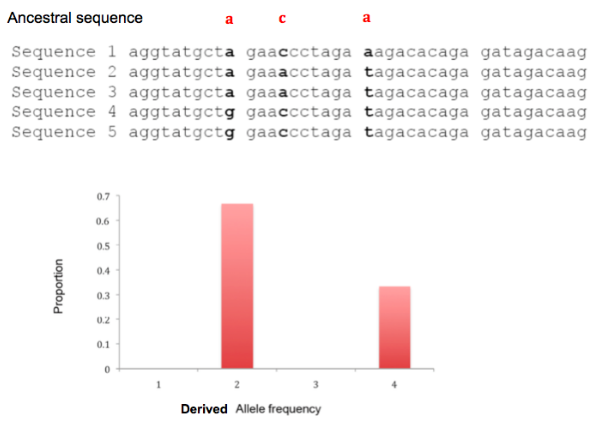
\includegraphics[width=0.7\textwidth]{Pics/sfs_count.png}
        \end{figure}

\end{frame}

%%%%%%%%%%%%%%%%%%%%%%%%%%%%%%%
\begin{frame}
\frametitle{Site frequency spectrum (SFS)}

	SFS under the neutral coalescent model for a sample of $n=11$ haploid individuals.

	\begin{figure}
                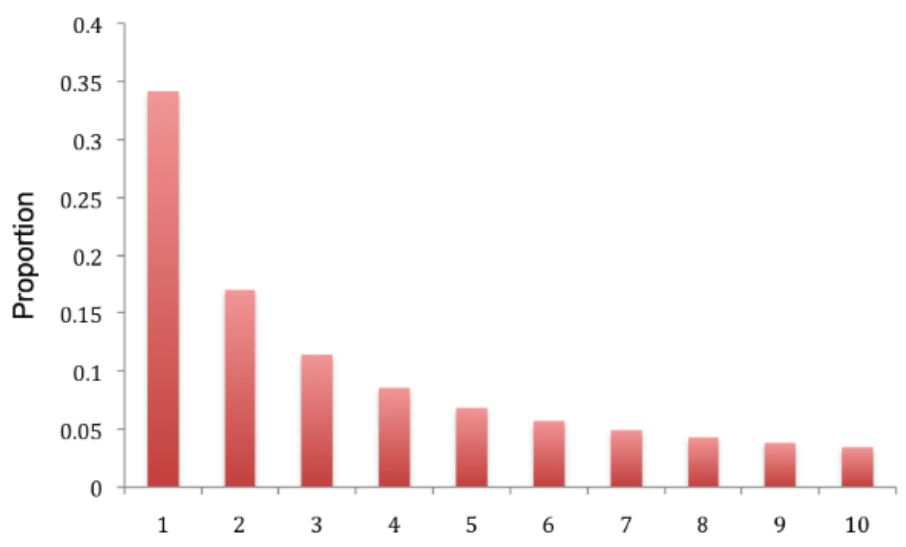
\includegraphics[width=0.7\textwidth]{Pics/sfs_exp.png}
        \end{figure}


\end{frame}

%%%%%%%%%%%%%%%%%%%%%%%%%%%%%%%
\begin{frame}
\frametitle{Site frequency spectrum (SFS)}

	From low-depth data:

        \begin{figure}
                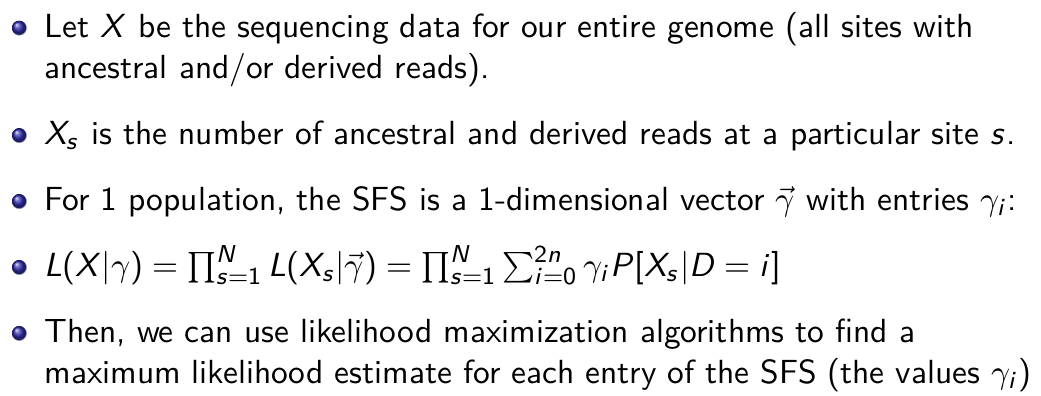
\includegraphics[width=\textwidth]{Pics/sfs_low.png}
        \end{figure}


\end{frame}

%%%%%%%%%%%%%%%%%%%%%%%%%%%%%%%

\begin{frame}
\frametitle{Exercise - 4}

	Calculate the SFS for each population and compare them.

	Estimate summary statistics (e.g. $\pi$, $\theta_W$) and make some comments on their different values.

	Advanced:
	
	Calculate the joint (2D) SFS and $F_{ST}$ in sliding windows.

\end{frame}





\section{Experimental design}

\begin{frame}

	Examples of optimal experimental design.

\end{frame}




%%%%%%%%%%%%%%%%%%%%%%%%%%%%%%%%%%%%%%%%%%%%%%%%%%%%%%%%%

\section*{ }
\frame{
 	\vbox{}
% 	\vfill
	\begin{centering}
	{\LARGE \usebeamercolor[fg]{title} Thank you for your attention}
	\par
	\end{centering}
}

\end{document}
